\documentclass{article} % use \documentstyle for old LaTeX compilers

%\usepackage[english]{babel} % 'french', 'german', 'spanish', 'danish', etc.
\usepackage{amssymb}
\usepackage{amsmath}
%\usepackage{txfonts}
%\usepackage{mathdots}
%\usepackage[classicReIm]{kpfonts}
\usepackage{graphicx}

% You can include more LaTeX packages here 


\begin{document}

%\selectlanguage{english} % remove comment delimiter ('%') and select language if required
\begin{center}
\Large\noindent POWER ELECTRONICS SYSTEMS FOR ELECTRIC VEHICLES
\begin{center}
EE -665
\end{center}

\large
\noindent \textbf{  REPORT ON :- }

\noindent THREE PHASE TWO LEVEL CONTROLLED BIDIRECTIONAL AC-DC CONVERTER WITH BIDIRECTIONAL DUAL ACTIVE BRIDGE ISOLATED CONVERTER SYSTEM
\begin{center}
\includegraphics*[width=4.25in, height=2.82in, keepaspectratio=false]{image1}
\end{center}

\noindent Submitted By:-

\noindent Prashant Verma 
                        
\noindent 214102107
                                          
\noindent Raghuwar Jee Jha

\noindent 214102112

\noindent Murtaza Gulamabbas Nimachwala 

\noindent        214102106                    

\noindent  Mallemputi Aravind

\noindent        214102509



\noindent   (Department of Electrical and Electronics Engineering)\\
\end{center}

\newpage

\Large\noindent 1. Objective\\
\noindent To simulate a three phase two level comtrolled  bidirectional ac-dc converter with bidirectional dual active bridge isolated converter system.The details of converter system amd othe rratings are given in the table below. The charging system has to be designed such that it charges from 75\% of State of Charge (SOC) to 85\% SOC. The charging system will charge the battery with\\
• 75\% to 80\% charging in constant current mode\\
• 80\% to 85\% charging in constant voltage mode  

\noindent specifications :- 


\begin{tabular}{|c|c|c|c|c|} 
\hline
s.no & specifications & valu & unit \\[0.5ex]
\hline
1 & input voltage & 6.6 ( L-L) & KV\\
\hline
2 & Frequency & 50 &  Hz \\
\hline 
3 & Battery Voltage & 400 & V \\
\hline
4 & Battery Energy Rating &  70 & kWhr \\
\hline
5 & Battery Charging Time ( 20 - 80 SOC) & 45 & min.  \\
\hline
6 & Input Power Factor & 1 & -- \\ 
\hline 
7 & Input Power Factor THD & 5\% & -- \\
\hline
8 & Output Voltage Ripple Of ac-dc converter & 5\% & -- \\
\hline

\end{tabular} \\


\Large\noindent{Design considerations}:-\\

      1. AC-DC CONVERTER 
    
  2. DC-DC CONVERTER:- \\
   
     The converter works in buck mode for charging the
battery. On the contrary, the converter works in boost mode.
Taking the buck mode as example, the control transfer
function for the converter can be expressed as :- \\

\begin{center}

$ G_{id(s)}= \frac{2V_{bus}(sC_O + \frac{1}{R_{load}})}{L_1 C_{o }{s^{2}}+\frac{L_1}{R_load}s +1}$ \\
\end{center}

Similarly, the control transfer function for the converter
in boost mode can be expressed as :-\\

\begin{center}


$G_{id(s))} = \frac{V_{bus}(sC_O + \frac{2}{R_{load}})}{L_1 C_{o }{s^{2}}+\frac{L_1}{R_load}s +2D'^{2}}$ \\

\end{center}




\noindent \includegraphics*[width=6.21in, height=6.29in, keepaspectratio=false]{image4}

\noindent 


\Large\noindent Control strategy :- 

\begin{enumerate}
\item  Current Closed-Loop Design:- 
\end{enumerate}

\noindent The inner current closed loop is used to keep the sinusoidal current input for system. It is obvious that the id and iq current loops are similar and symmetrical. The control diagram is shown below.\\
\begin{center}
\noindent \includegraphics*[width=6.24in, height=2.68in, keepaspectratio=false]{image7}



\end{center}

\begin{figure}
\includegraphics[scale=0.23]{raghu01.jpg}
\end{figure}







\noindent  $T_s$ is the sample period of current loop; Kip and KiI are the proportional and integration coefficients of PI regulator, respectively; and $K_{pwm}$ is the equivalent gain of the three-phase pulse width modulated converter.
\noindent Now this closed loop can be  simplified into the following  transfer function :- \\
\begin{center}

$\frac{1}{{1+{\frac{R.\tau_i}{K_{ip}. K_{pwm}}}}s+{\frac{1.5 T_sR. \tau_i s^{2}}{K_{ip}. K{wmp}}}}$\\
 \end{center}
 


\noindent 

\noindent Using the above transfer function we plotted the bode plot for various values of of K${}_{p\ }$\& K${}_{i\ }$.\\

\noindent \includegraphics*[width=5.90in, height=2.72in, keepaspectratio=false]{image2}\\
Bode diagram for different values for proportional and integration coefficients. \\

\Large CALCULATIONS:- \\

    1. FILTER CALCULATIONS:-\\
    
      A. Capacitor,C calculation :- \\
      
    $  \frac{{V_{L-L}}^2}{3.X_c} = Q $ \\
    Q is 5\% of the rated power. \\
   $ therefore, X_{c} =\frac{{V_{l-l}}^2}{3 Q}$ \\ 
   
   Solving this we get ,  \\
   
  $  C = \frac{3 * 2800}{ 2 * \pi * 50 * 6.6 * 6.6 * 10^{6}} $ \\
   therefore, C = 500 micro Farad. \\
   
     B. Inductor calculations :-  \\
    $  L_{1} = L_{2} = \frac{V_{dc}}{4 *h* f_{sw}} \\ $
      here, 2h = 40\% of rated current \\
$      h= 0.4* \frac{56000}{6600 * 1.732} \\ $
       h= 0.98 \\
$putting values in the expression of L_{1} and L_{2} ,we get \\$
       
$       L_{1} =L_{2} = 0.5mH $ \\

      C.  DAB CALCULATIONS :- \\
       (i) inductor calculation :- \\
       
  $     \Delta I_l = \frac{V_o (1-D)}{L . f_s} $ \\
      $   2\% = \frac{0.02 *140*10000}{400* 0.5} $ \\
    $  therefore       ; L = 2mH . $ \\
    
       (ii) Capacitor Calculation :- \\
       $ \Delta = \frac{V_o (1-D)}{8.L.C. f^{2}} 4 \\ $
      $ 0.025 * 400 = \frac{400 * 0.5}{8* 0.001 *2*C*10000 L} \\ $
    $   C = 190 \mu F. $ \\
   
      
      
    
       

\noindent Simulation and experiment results 

\begin{enumerate}
\item  Simulation results : - Simulation is established in MATLAB.\\ System configuration is shown in figure 1, and detailed parameters  are in table. 
\end{enumerate}




\noindent 

\noindent 

\noindent \includegraphics*[width=5.89in, height=2.69in, keepaspectratio=false]{image3}\\
\begin{center}



\begin{figure}
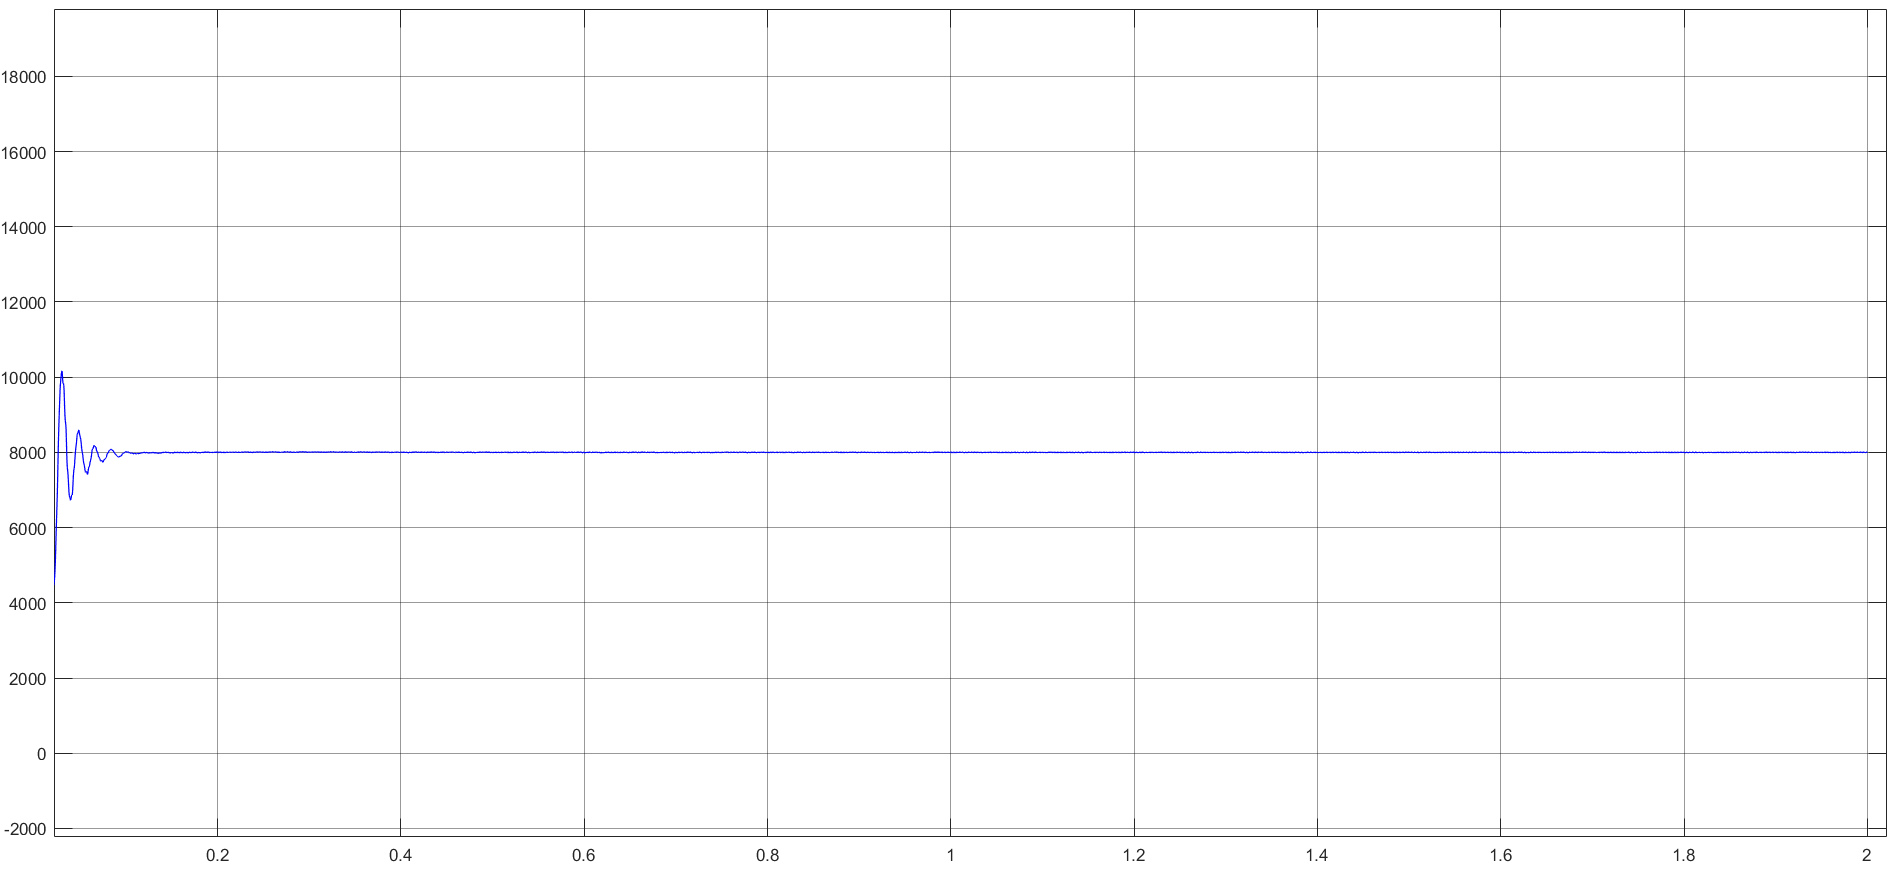
\includegraphics[scale=0.30]{AC to DC voltage.png}
\end{figure}
 
 Discharging output \\
 \begin{figure}
 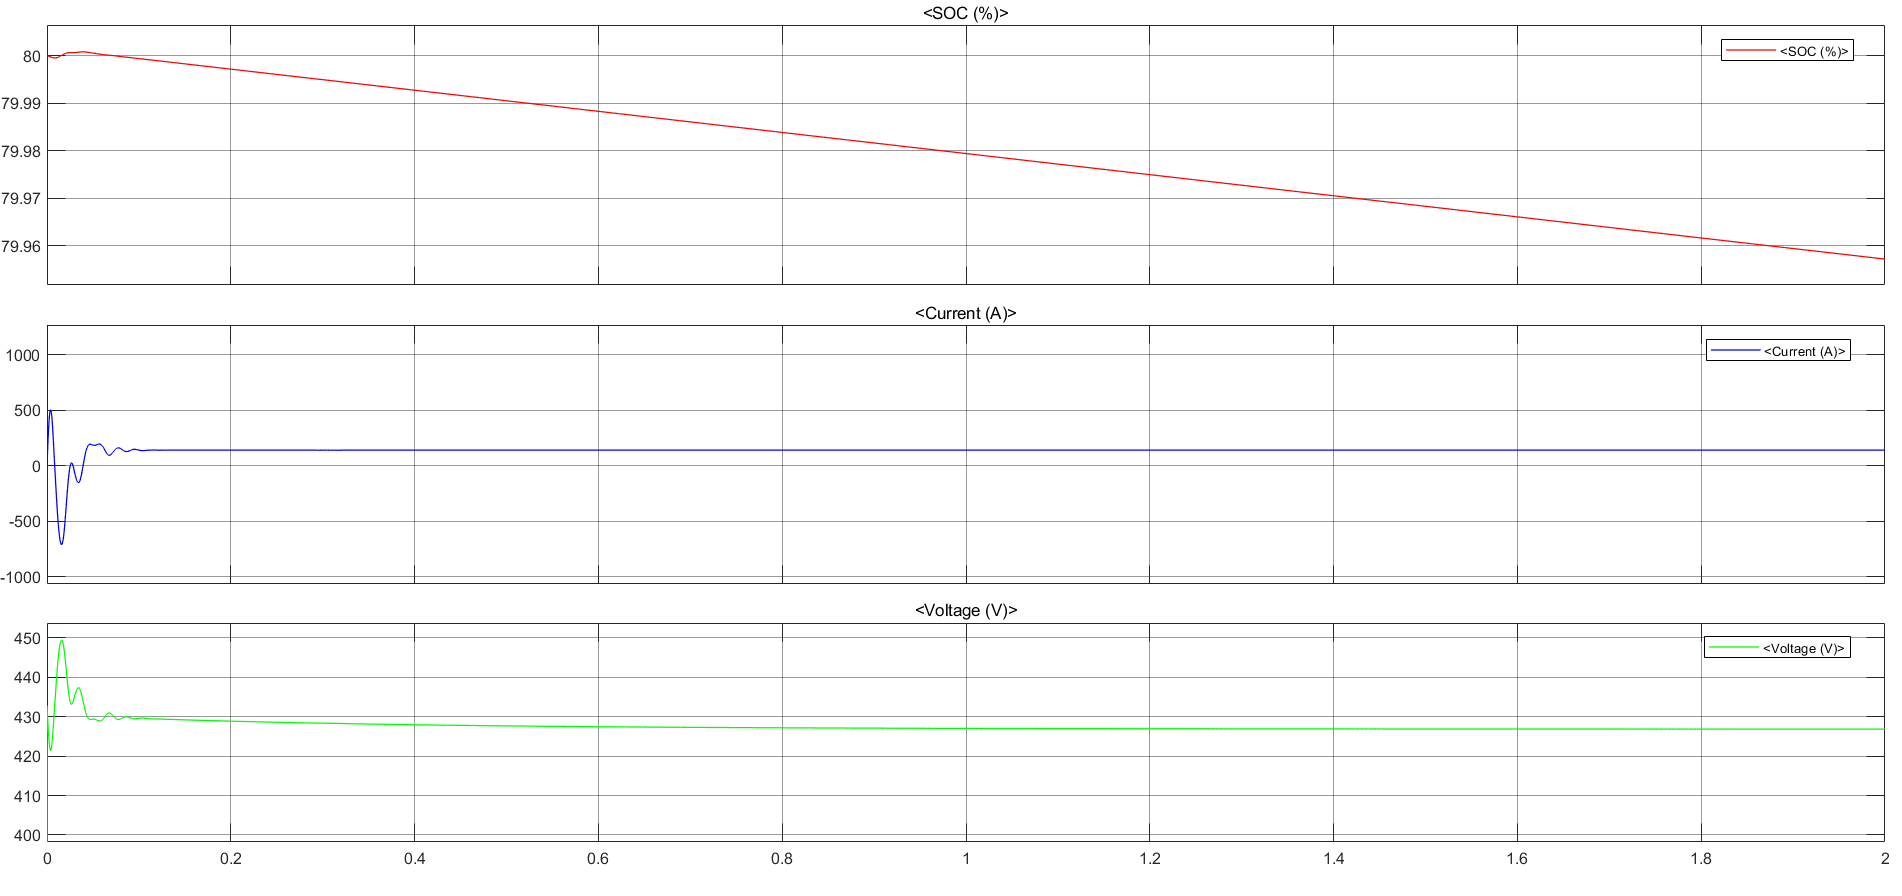
\includegraphics[scale=0.30]{discharge.png}
 \end{figure}

\begin{figure}
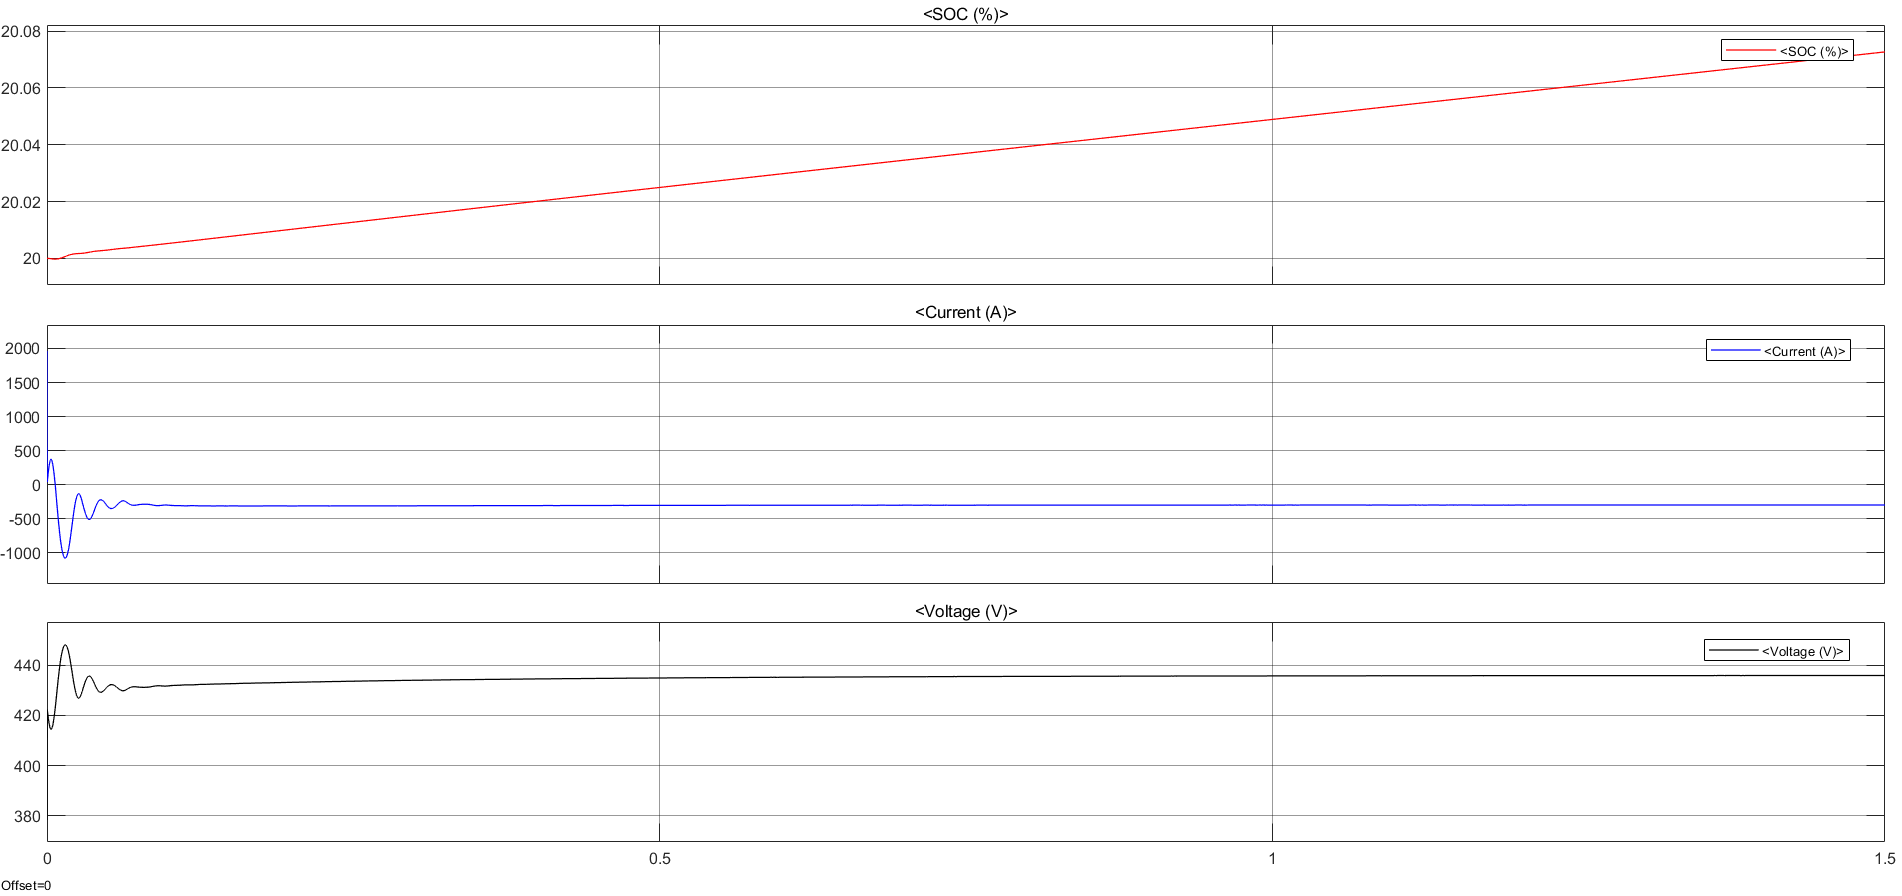
\includegraphics[scale=0.30]{charging.png}
\end{figure}

\begin{figure}
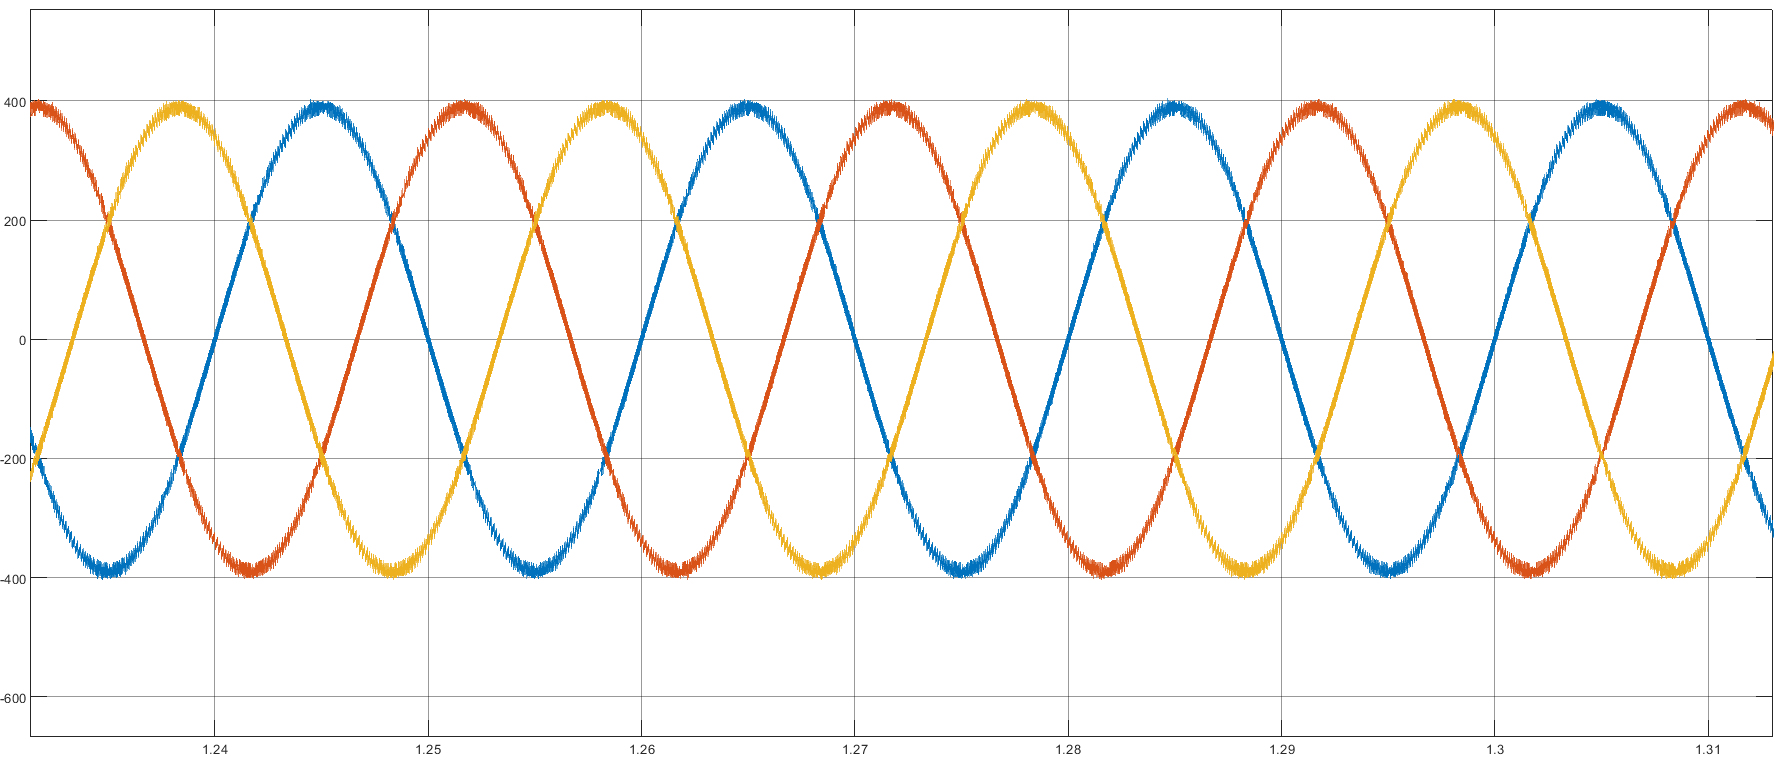
\includegraphics[scale=0.30]{Grid Current.png}
\end{figure}

\end{center}


 

\end{document}







 
 




\end{document}


